% copyright arturo salinas-aguayo 2025
\documentclass[12pt]{article}

\usepackage{graphicx} \usepackage{subcaption} \usepackage{amsmath}
\usepackage{siunitx} \usepackage{array} \usepackage{amsfonts}
\usepackage{fancyhdr} \usepackage{geometry} \usepackage{circuitikz}
\usepackage{caption} \usepackage{karnaugh-map} \usepackage{bm}
\usepackage{float}

\geometry{letterpaper, margin=1in} \graphicspath{ {../../images/} }

% Header and Footer
\pagestyle{fancy} \fancyhf{} \fancyhead[L]{ECE 3201 - Lab 01: Half-Wave and Full-Wave Rectification}
\fancyhead[R]{\thepage} \setlength{\headheight}{15pt}

\author{Arturo Salinas-Aguayo} \title{Lab 01: Half-Wave and Full-Wave Rectification}

% theorem set
\newtheorem{example}{Example}
% Example block environment
\newenvironment{examp} {\vspace{0.5cm} \hrule \vspace{0.5cm}
	\begin{example}} {\hrule \vspace{0.5cm}
\end{example}}

\begin{document}
\newcommand{\closure}[2][3]{%
	{}\mkern#1mu\overline{\mkern-#1mu#2}}
\newcommand\ncoverline[1]{\mkern1mu\overline{\mkern-1mu#1\mkern-1mu}\mkern1mu}
% Title Page
\begin{titlepage}
	\centering \vspace*{3cm} \huge\textbf{Lab 01: Half-Wave and Full-Wave
		Rectification}\\

	\vspace{5cm} \Large\textbf{Arturo Salinas-Aguayo}\\
	\normalsize ECE 3201 Electronic Circuit Design and Analysis\\
	Dr. Mehdi Anwar\\
	Electrical and Computer Engineering Department\\
	\vfill 
\includegraphics[scale=0.1]{uconnlogo}\\
	College of Engineering, University of Connecticut\\
	\scriptsize{Coded in \LaTeX} \vspace*{1cm}
\end{titlepage}

\tableofcontents

\newpage

\section{Abstract}
This lab introduced the concept of rectification using semiconductor diodes as
nonlinear circuit elements. Half-wave and full-wave rectifiers were
constructed, measured, and analyzed to demonstrate the conversion of
alternating current (AC) into direct current (DC). The effect of diode forward
voltage drop and peak inverse voltage (PIV) were considered, and ripple
reduction techniques were explored using filter capacitors. Experimental
results were compared to theoretical predictions, and discrepancies were
explained in terms of practical component tolerances and non-ideal diode
behavior. The lab provided a foundational understanding of rectifier operation,
efficiency, and filtering, which are essential for power electronics
applications.

\newpage
\section{Introduction}
A diode is a two-terminal nonlinear device that ideally conducts with
negligible drop when forward-biased and blocks when reverse-biased. Real
silicon diodes exhibit a forward drop near \SI{0.7}{V} and finite reverse
leakage, which directly impact rectifier performance. These one-way conduction
properties (mechanically analogous to a check valve) enable conversion of AC to
unidirectional DC. In this lab we use half-wave, bridge, and center-tap
full-wave rectifiers to quantify the effects of diode forward drop, PIV, and
$RC$ filtering on average output and ripple.

\begin{figure}[H] \centering 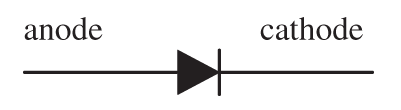
\includegraphics[width=0.5\textwidth]{lab1diode}
	\caption{The Schematic Diagram of a Diode} \label{fig:diode}
\end{figure}

Think of the diodes mechanical analog being the check-valve. A check-valve in a
fluid system allows the fluid to flow in one direction only, with a mechanical
gate swinging down preventing the backflow of fluid in the improper direction.
The diode acts very much the same way. These characteristics can be exploited
to produce circuitry that was previously not possible with the components of
ECE 2001 such as rectification circuits, voltage-shifting circuits, and
voltage-limiting currents.



\section{Objective} The objective of this lab is to investigate the operation
of half-wave and full-wave rectifier circuits using diodes, and to analyze
their ability to convert alternating current (AC) signals into direct current
(DC). We  will construct and measure different rectifier configurations,
compare theoretical and experimental results for output voltage and ripple, and
evaluate the effects of circuit parameters such as diode forward voltage drop,
peak inverse voltage (PIV), and filter capacitors on rectifier performance.

\section{Theory}

Rectification is the process of converting an alternating current (AC) signal
into a direct current (DC) signal using semiconductor diodes. A diode is a
nonlinear device that ideally behaves as a short circuit when forward biased
and as an open circuit when reverse biased. In practice, a forward voltage drop
of approximately $0.7\,\text{V}$ for silicon diodes must be considered.

\subsection{Half-Wave Rectifier} In a half-wave rectifier, the diode conducts
only during the positive half-cycle of the input sinusoidal signal. During the
negative half-cycle, the diode is reverse biased, and the output voltage is
zero. For an ideal diode, the instantaneous output is
\[
	v_{o}(t) = v_{i}(t), \quad 0 < \omega t < \pi,
\]
and
\[
	v_{o}(t) = 0, \quad \pi < \omega t < 2\pi.
\]
Accounting for the diode forward voltage drop $V_D$, the output becomes
\[
	v_{o}(t) = v_{i}(t) - V_D, \quad v_{i}(t) > V_D.
\]
The average (DC) output voltage is approximated as
\[
	V_{DC} \approx \frac{V_{m}}{\pi} - \frac{V_D}{2},
\]
where $V_{m}$ is the peak input voltage. The main limitation of the half-wave
rectifier is its low efficiency since only half of the input waveform
contributes to the output.

\subsection{Full-Wave Rectifier} In a full-wave rectifier, both halves of the
input waveform are utilized. This can be achieved using either a center-tapped
transformer with two diodes or a four-diode bridge rectifier. In both cases,
the output waveform is unidirectional, effectively doubling the frequency of
the rectified signal. The average output voltage for an ideal diode is
\[
	V_{DC} \approx \frac{2V_{m}}{\pi}.
\]
Compared to the half-wave rectifier, the full-wave rectifier provides a higher
average DC voltage and improved efficiency.

\subsection{Filtering}
The output of a rectifier is not a constant DC value but contains ripples. To
reduce ripple voltage, a filter capacitor is connected across the load
resistor. The capacitor charges quickly to the peak value of the rectified
waveform and discharges slowly through the load during the non-conducting
period of the diode. The resulting ripple voltage can be approximated as
\[
	V_{r} \approx \frac{V_{p}}{fRC},
\]
where $V_{p}$ is the peak output voltage, $f$ is the frequency of the rectified
waveform, $R$ is the load resistance, and $C$ is the filter capacitance. For
effective filtering, the condition $RC \gg T$ (where $T = 1/f$) must be
satisfied.

\subsection{Peak Inverse Voltage (PIV)} The peak inverse voltage is the maximum
reverse bias voltage that a diode must withstand during operation. In a
half-wave rectifier, the PIV is equal to the peak input voltage $V_{m}$. In a
bridge rectifier, each diode experiences a PIV of $V_{m}$, whereas in a
center-tap full-wave rectifier, the PIV is $2V_{m}$. Thus, diode selection must
ensure that the breakdown voltage rating exceeds the PIV by a safe margin.


\section{Experimental Procedures}
\subsection{Circuit One}
The first circuit analyzed was a simnple half-wave rectifier using a silicon
diode outlined in Figure \ref{fig:cir1}.
This involved an input signal of $10V_{pp}$ at 1KHz from the signal generator
and a 1N457 diode.

\begin{figure}[H] \centering 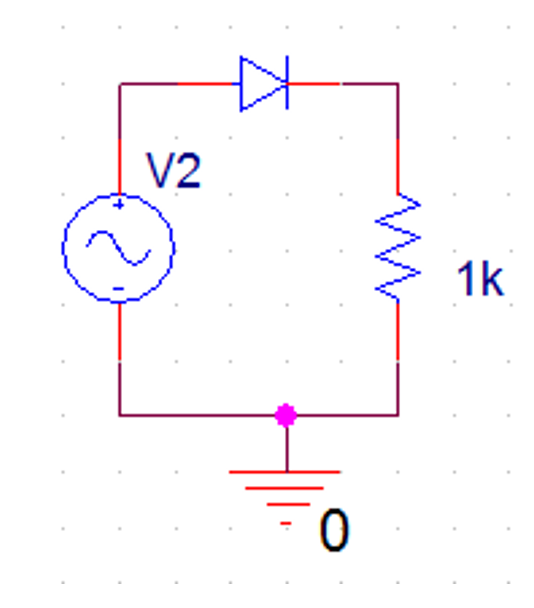
\includegraphics[width=0.5\textwidth]{lab01/cir1}
	\caption{A Half-Wave Rectifier Circuit} \label{fig:cir1}
\end{figure}

\subsection{Circuit Two}
The second circuit analyzed was a Full-Wave Rectifier and involved a slightly
more complicated test procedure.
The full wave rectifier circuit also utilized the 1N457 diode, but this time 4
were used in order to obtain the correct charactersics of a full-wave
rectification circuit. This also employed the use of a transfomer circuit that
was tuned to obtain $120V_{rms}$ from the wall socket at 60Hz and transform
that down via a secondary winding to an obtained voltage of $16.0V_{rms}$. The
circuit schematic is shown in Figure \ref{fig:cir2}

\begin{figure}[H] \centering 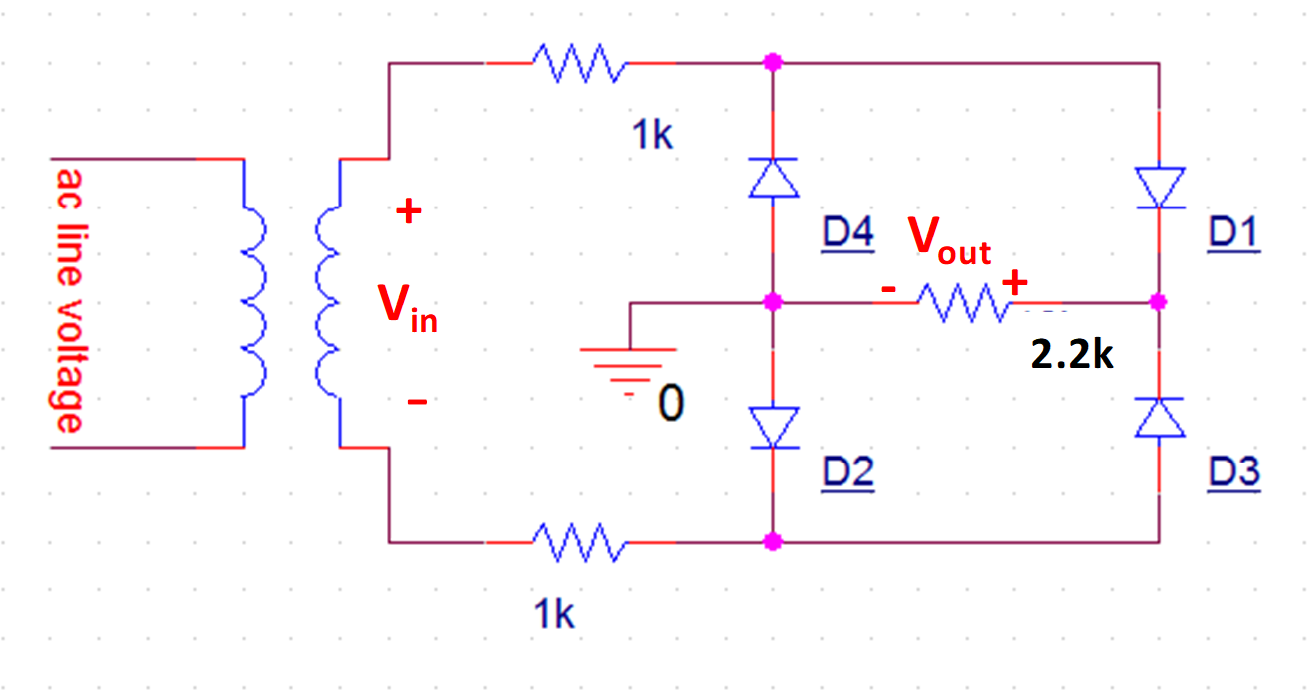
\includegraphics[width=0.5\textwidth]{lab01/cir2}
	\caption{A Full Bridge Rectifier Circuit} \label{fig:cir2}
\end{figure}

\subsection{Circuit Three}
The third circuit involved a more simplified paradigm of the Full Wave
rectification circuit, this time only employing one half of the 1N457 diode.

The same circuit specifications were used, but this time the center tap of the
transformer was regarded as reference. This effectively splits the voltage felt
at the terminals in half as shown in the following Results section. The circuit
is shown in Figure \ref{fig:cir3}.
\begin{figure}[H] \centering 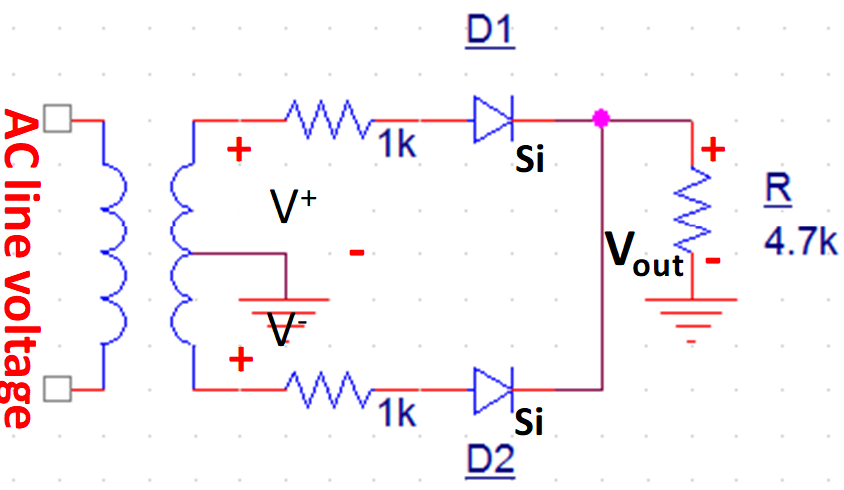
\includegraphics[width=0.5\textwidth]{lab01/cir3}
	\caption{A Full Wave Center Tap Configured Circuit} \label{fig:cir3}
\end{figure}

\subsection{Circuit Four}
The final circuit involved a design skill and the use of some formulas that
were previously mentioned in the Theory section. Using a target ripple voltage
of 0.8V with an input of a $5V_{pp}$ sine wave at 60Hz, a resistance and
capacitance value had to be chosen such that these design conditons hold true.
The circuit is shown in Figure \ref{fig:cir4}.

\begin{figure}[H] \centering 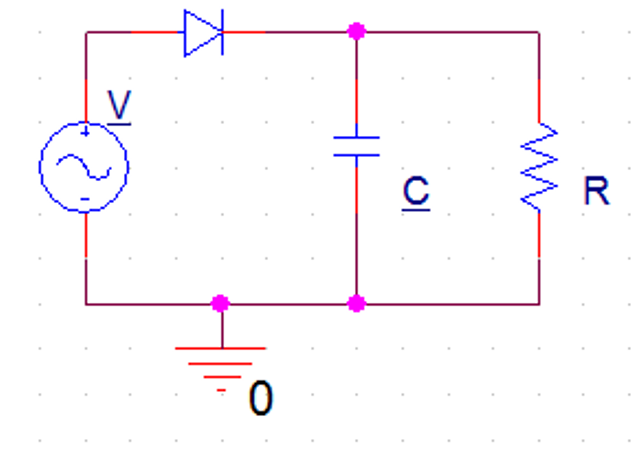
\includegraphics[width=0.5\textwidth]{lab01/cir4}
	\caption{Rectifier Circuit with Filtering Capacitor} \label{fig:cir4}
\end{figure}

\section{Results}
\subsection{Circuit One}

The input signal can be seen in Figure \ref{fig:cir1input} and the respective
output signal can be seen in Figure \ref{fig:cir1output}. The behavior follows
expectations with the diode obtaining some amount of voltage during the drop.
Notice the peak input voltage tops out at 4.793V, while the peak output voltage
tops out at 3.914V.

\begin{figure}[H] \centering 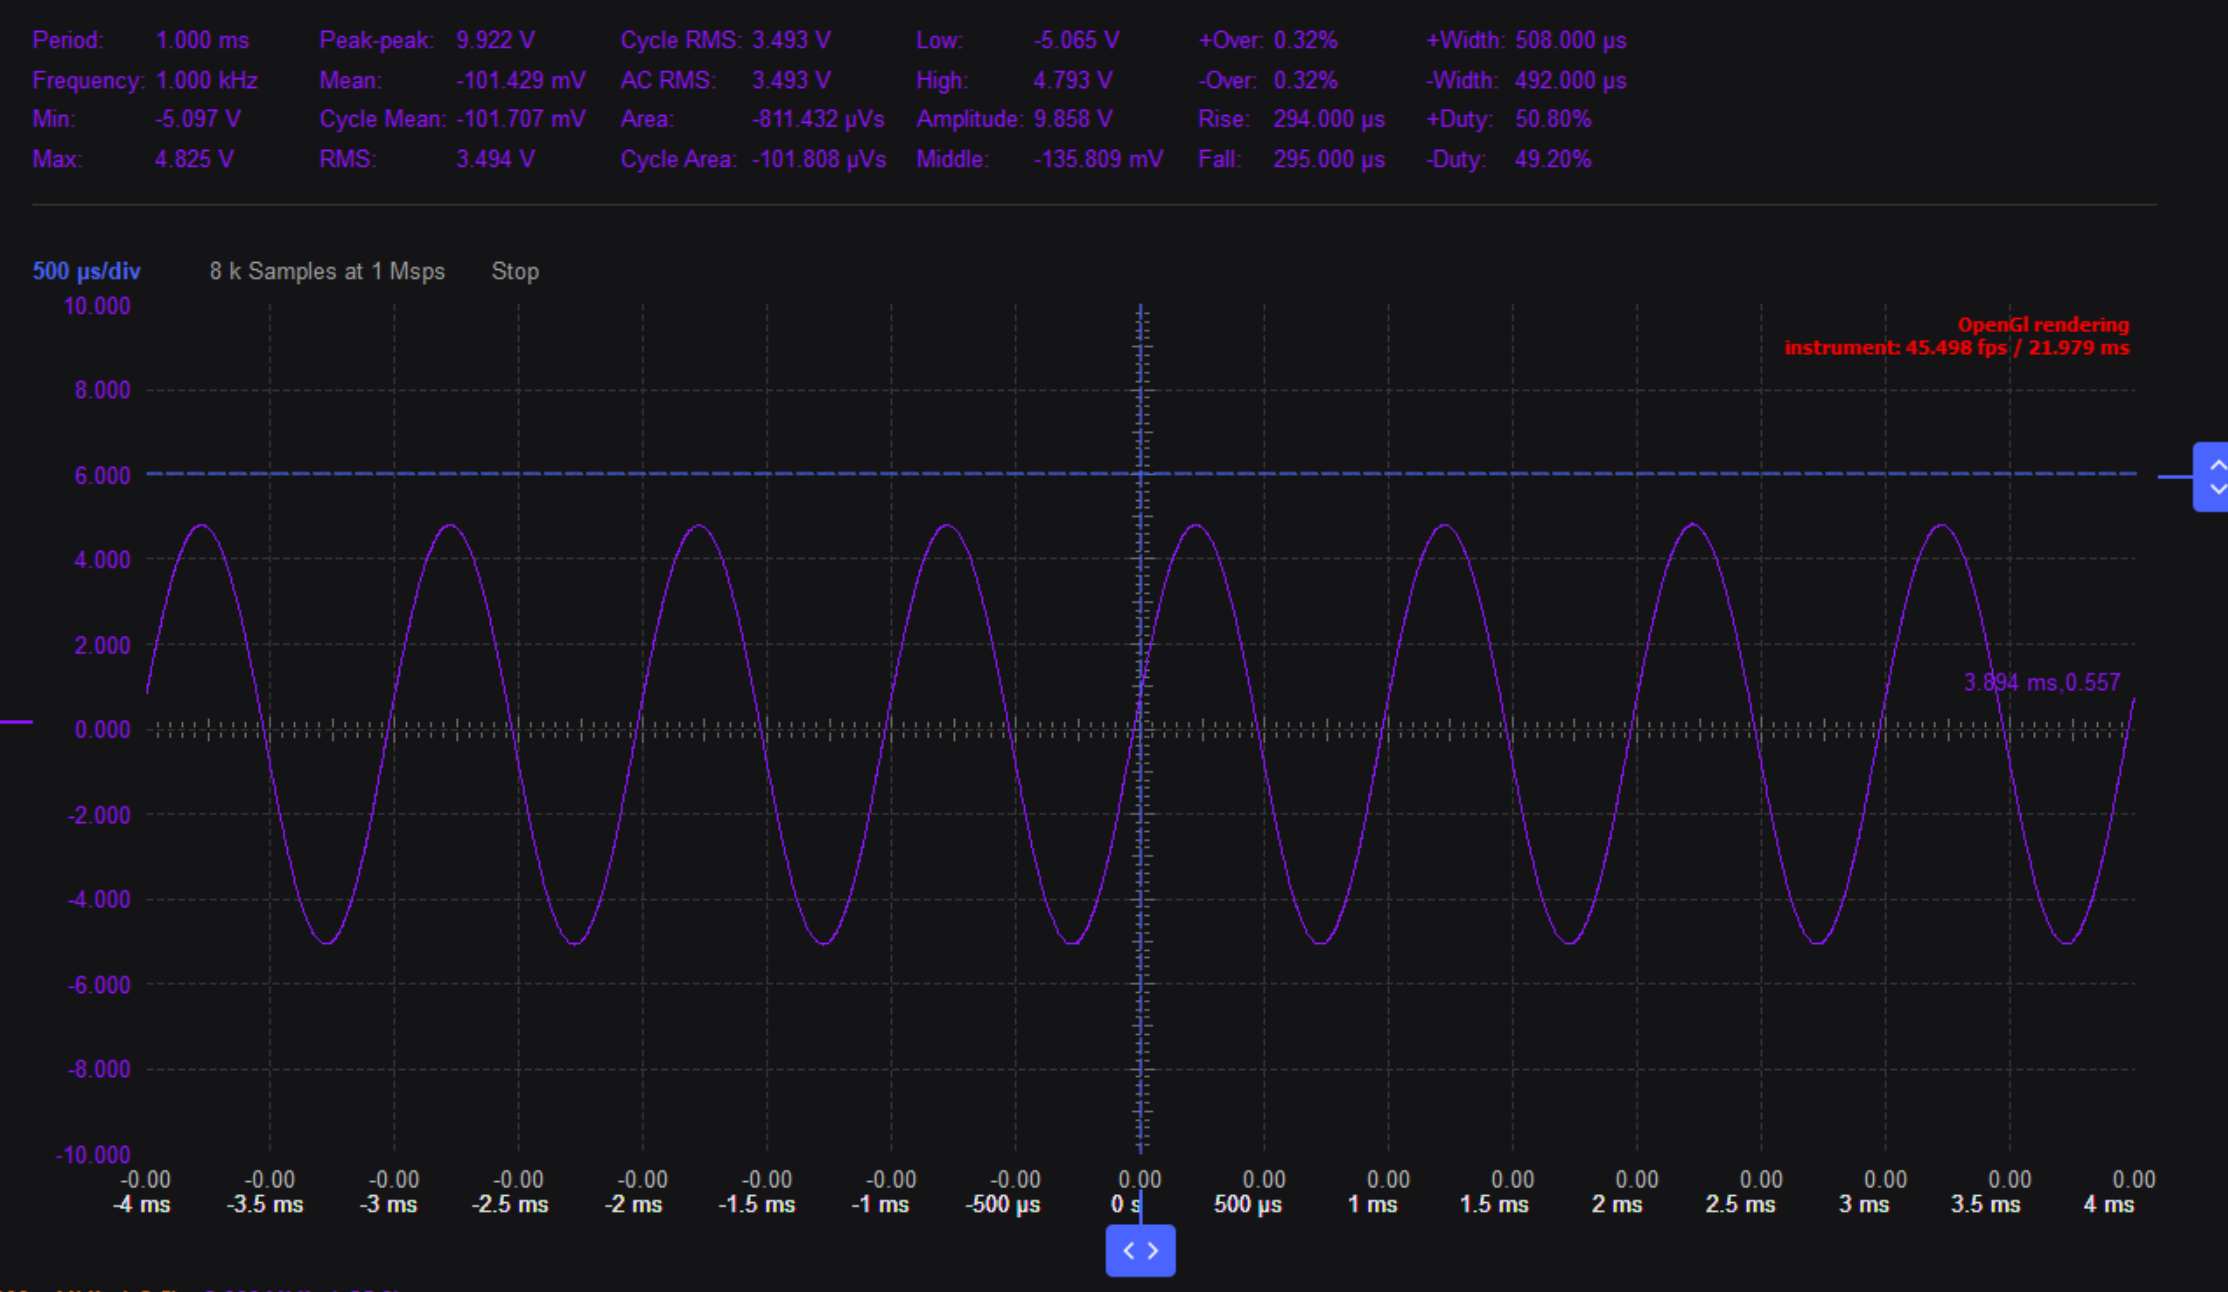
\includegraphics[width=1.0\textwidth]{lab01/cir1input}
	\caption{Input Waveform to Circuit One} \label{fig:cir1input}
\end{figure}

\begin{figure}[H] \centering 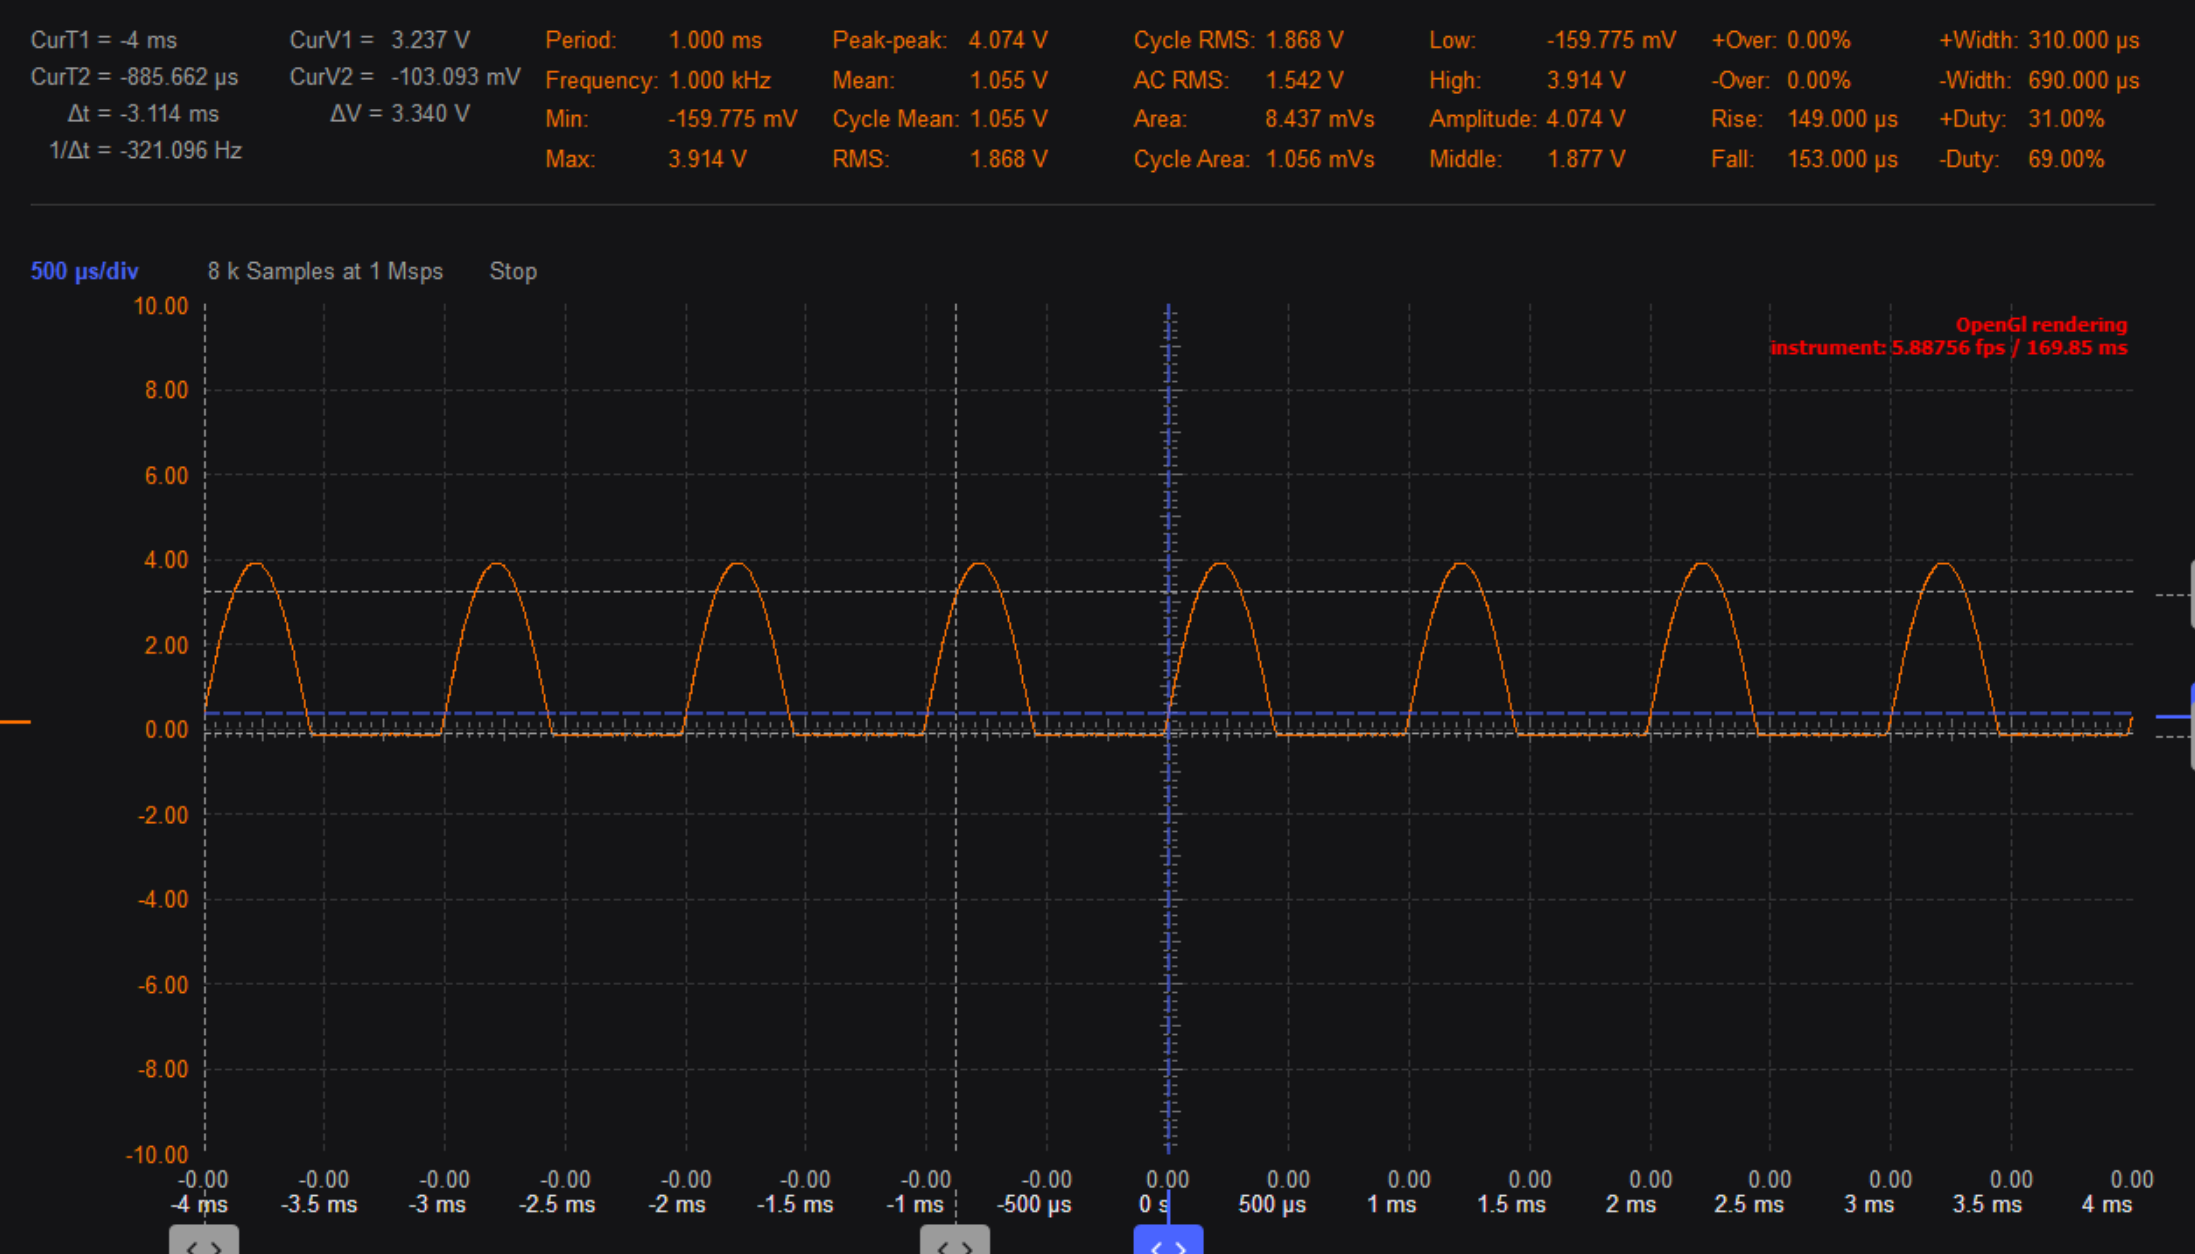
\includegraphics[width=1.0\textwidth]{lab01/cir1output}
	\caption{Output Waveform to Circuit One} \label{fig:cir1output}
\end{figure}

Subtracting the two and accounting for the DC offset in the output gives
\[
	4.793\text{ V} - \bigl(3.914\text{ V} + 0.1598\text{ V}\bigr) = 0.7192\text{ V}.
\]
This aligns with the expected forward drop plus loading effects.

Taking the RMS voltage off of the resistor, the following was obtained:
\[
	V_{R_{rms}}\text{ Multimeter = }1.530 V_{rms}\\
\]
\[
	V_{R_{rms}}\text{ Oscilloscope = }1.878 V_{rms}\\
\]
The oscilloscope reports \emph{true} RMS (DC + AC):
\[
	V_{\text{RMS,scope}} = 1.878\ \text{V}.
\]
The multimeter reports the \emph{AC-only} RMS, these are related by
\[
	V_{\text{RMS,scope}}^{2} = V_{DC,\text{meas}}^{2} + V_{\text{RMS,AC}}^{2}
	\;\;\Longrightarrow\;\;
	V_{\text{RMS,AC}} = \sqrt{V_{\text{RMS,scope}}^{2} - V_{DC,\text{meas}}^{2}}.
\]
Substituting the measurements,
\[
	V_{\text{RMS,AC}} \approx \sqrt{(1.878)^2 - (1.055)^2} \approx 1.55\ \text{V},
\]
which agrees closely with the multimeter reading
\[
	V_{R,\text{RMS}}(\text{multimeter, AC}) = 1.530\ \text{V}.
\]
For reference, the ideal half-wave total RMS is \(V_{p,\text{out}}/2 \approx 3.914/2 = 1.957\ \text{V}\),
reasonably close to the scope’s \(1.878\ \text{V}\) given non-idealities.

For an \emph{ideal} half-wave rectifier, \(V_{DC} \approx V_{p,\text{out}}/\pi\), so
\[
	V_{DC,\text{ideal}} \approx \frac{3.914}{\pi} \approx 1.246\ \text{V}.
\]
The measured mean was \(1.055\ \text{V}\), lower as expected due to the diode drop and the slightly
reduced conduction angle (the diode only conducts while \(v_i(t) > V_D\)).

The 1N4148 diode is a completely different diode than the one used in this
experiment. Looking at the data sheet, the 1N4148 has a reverse breakdown
voltage of 100V. The Peak Inverse Voltage for this circuit, or PIV, is simply
5V, which is $5\%$ of this rating. Therefore, it heavily exceeds this
requirement.

Upon decreasing the amplitude to $2V_{pp}$, the following differences are shown:

\begin{figure}[H] \centering 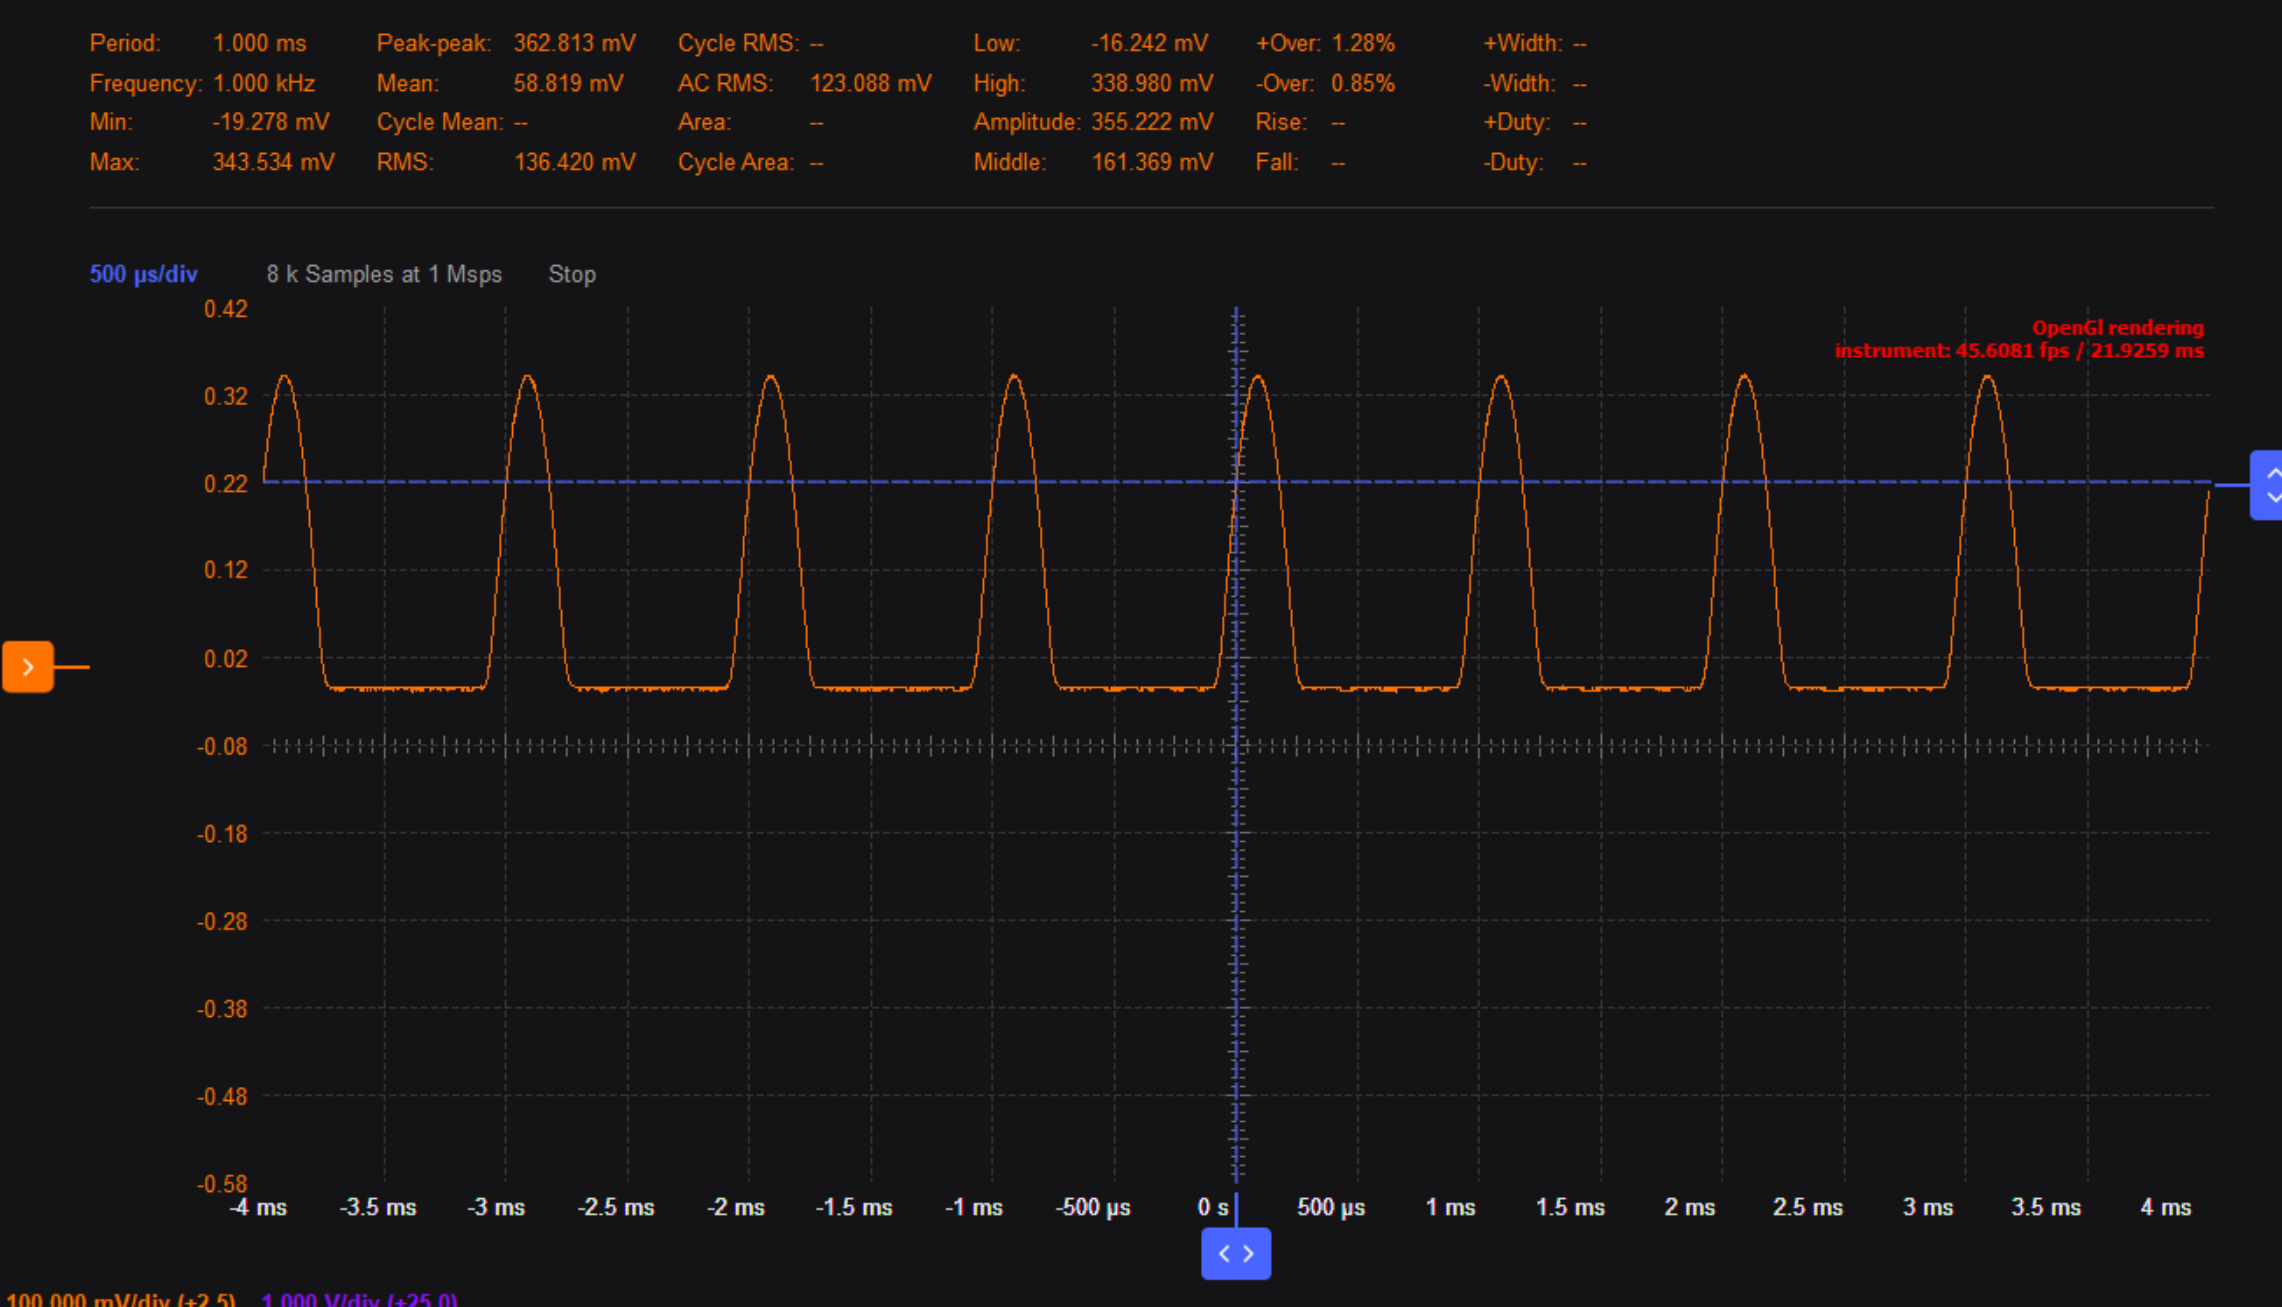
\includegraphics[width=0.8\textwidth]{lab01/cir1output2}
	\caption{Output Waveform to Circuit One @ $2V_{pp}$} \label{fig:cir1output2}
\end{figure}

VR @2V-measured becomes $58.819mV$ and the calculated VR becomes $107.6mV$.
Because \(V_D\) is a small fraction of the peak (\(0.7/5 \approx 14\%\)), the ideal formula
\(V_{DC}\approx V_p/\pi\) remains accurate and the conduction angle is near \(\pi\). At
\(2\ \mathrm{V_{pp}}\) (\(V_p=1\ \text{V}\)), \(V_D/V_p\) is large (\(\approx 70\%\)), the conduction angle
shrinks, and non-idealities (diode curve, meter resolution, waveform distortion) dominate, pulling the
measured DC below the ideal estimate.
\subsection{Circuit Two}
Circuit two, shown in Figure \ref{fig:cir2} involved taking measurements of the
output resistor again, however the characteristics now show a full wave
rectification circuit output. First, the input voltage shown in
\ref{fig:cir2input} shows a $16V_{rms}$ reading off of the transformer windings
provided by the lab.

\begin{figure}[H] \centering 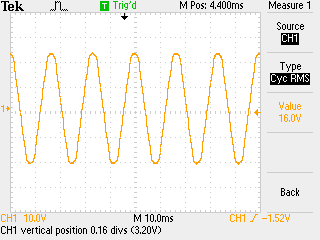
\includegraphics[width=0.8\textwidth]{lab01/cir2input.png}
	\caption{Input Waveform to Circuit Two} \label{fig:cir2input}
\end{figure}

The output, as measured from the resistor displayed both sides of the input
sine wave, but on the positive side. As there are four diodes now in a bridge
configuration, half of the diodes `fire` when the input sine wave is in the
positive half of conduction, and the other half `fire` when the signal is in
the negative half. This allows for the entire signal to pass through as
positive and for better circuit efficiency at the cost of the additional
components needed to build the circuit. The Mean and Max outputs of these
signals are shown in Figures \ref{fig:cir2outputmax} and
\ref{fig:cir2outputmean} respectively.


\begin{figure}[H] \centering 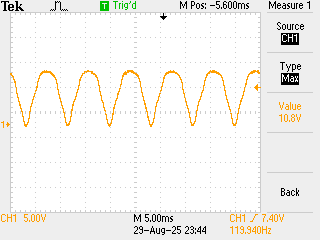
\includegraphics[width=0.8\textwidth]{lab01/cir2outputmax.png}
	\caption{Output Max Waveform of Circuit Two} \label{fig:cir2outputmax}
\end{figure}

\begin{figure}[H] \centering 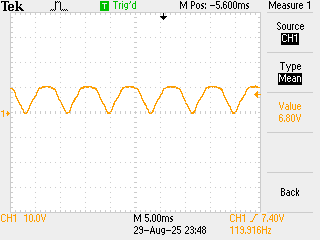
\includegraphics[width=0.8\textwidth]{lab01/cir2outputmean.png}
	\caption{Output Mean Waveform to Circuit Two} \label{fig:cir2outputmean}
\end{figure}

This resulted in the following values:
\[
	V_{IN} = 15.9V
\]
\[
	V_{{OUT}_{MAX}} = 10.8V
\]
\[
	V_{{OUT}_{DC}} = 6.8V
\]
Intuitively, these all make sense. On each half of the signal (positive and
negative) there are now two diodes which drop the voltage when they are forward
biased. Setting these to approximately 0.7V mentally, the max peak voltage
alongside the added resistance from the resistor make the max voltage as
expected. The DC Component of the circuit is also closer to the average as each
period now has both halves of the sine wave included, allowing use of the mean
measurement of the oscilloscope to be accurate compared to before in Circuit
One.
\subsection{Circuit Three}
Circuit Three introduced the use of the center tap of the transformer. The center tap effectively cuts the transformer into two halves right down the center.

This is shown in the input waveforms. The positive half is shown in Figure \ref{fig:cir3pos} and the negative half is shown in Figure \ref{fig:cir3neg}.

\begin{figure}[H] \centering 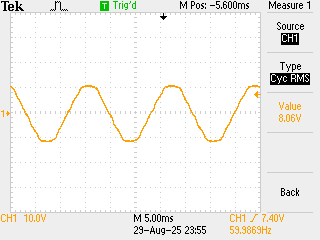
\includegraphics[width=0.8\textwidth]{lab01/cir3pos.png}
	\caption{Positive Transformer Half Side Input to Circuit 3} \label{fig:cir3pos}
\end{figure}

\begin{figure}[H] \centering 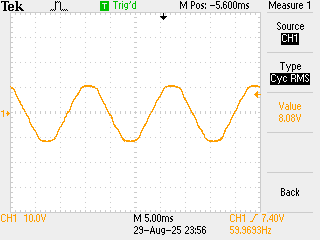
\includegraphics[width=0.8\textwidth]{lab01/cir3neg.png}
	\caption{Negative Transformer Half Side Input to Circuit 3} \label{fig:cir3neg}
\end{figure}

This results in:
\[
	V_{IN+} = 8.06V_{RMS}
\]
\[
	V_{IN-} = 8.08V_{RMS}
\]
\[
	V_R = 6.03V_{RMS}
\]
The output waveform can be seen in Figure \ref{fig:cir3out}.
\begin{figure}[H] \centering 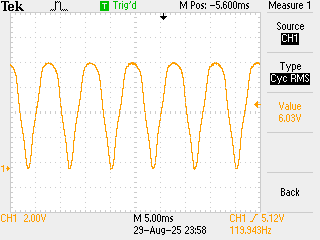
\includegraphics[width=0.8\textwidth]{lab01/cir3out.png}
	\caption{Circuit Three Output Waveform} \label{fig:cir3out}
\end{figure}
Which is very similar indeed to Circuit Two. One could say that the outcome is the same, but with different physical characteristics and costs associated with each circuit. I'll delve into some details here.

The output, as taken from the resistor shows a response similar to the one in Circuit Two, but with the PIV doubled. This center-tapped full-wave recitifier behaves like a half-wave rectifier in the top half, and another one in the bottom half, phase shifted so that the output is a similarly clean, energetic output waveform.

In terms of the output voltage, since there is one less diode on each half of the input waveform, that means that there is only one (0.7V) drop in potential voltage on each half of conduction compared to Circuit Two.

\[
	V_{out,\;\text{center-tap}} \approx V_{m} - V_{D}
\]

\[
	V_{out,\;\text{bridge}} \approx V_{m} - 2V_{D}
\]
To explain further on the aspect of the PIV calculation, consider:
\[
	PIV = 2V_S - V_D
\]
compared to Circuit Two's:
\[
	PIV = V_S - 2V_D + V_d = V_S - V_D
\]
The PIV is about half the value for the full-wave rectifier with a center-tapped tranformer!
\subsection{Circuit 4}

For the rectifier with filter capacitor shown in Fig.~\ref{fig:cir4}, the ripple voltage
is approximated by
\[
	V_{r} \approx \frac{V_{p}}{fRC},
\]
where $V_{p}$ is the peak input voltage, $f$ is the frequency, $R$ is the load resistance,
and $C$ is the filter capacitance.

Given:
\[
	V_{p} = \frac{5\,\text{V}_{pp}}{2} = 2.5\,\text{V}, \quad
	f = 60\,\text{Hz}, \quad
	V_{r} = 0.8\,\text{V},
\]
\[
	R = 2.2\,\text{k}\Omega, \quad
	C = 22\,\mu\text{F}.
\]

Substituting into the ripple equation:
\[
	V_{r} = \frac{2.5}{60 \times 2200 \times 22 \times 10^{-6}},
\]
\[
	V_{r} = \frac{2.5}{2.904} \approx 0.86\,\text{V}.
\]

Thus, the calculated ripple voltage with the chosen values is
\[
	V_{r} \approx 0.86\,\text{V},
\]
which is close to the design target of $0.8\,\text{V}$.

Using the oscilloscope, the measured ripple voltage was found to be
\[
	V_{r,\text{measured}} \approx 0.96\,\text{V}.
\]
as shown in Figure \ref{fig:cir4output}.

\begin{figure}[H] \centering 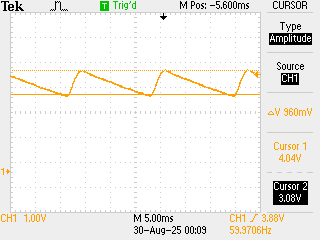
\includegraphics[width=0.8\textwidth]{lab01/cir4output.png}
	\caption{The Designed Circuit Ripple Voltage} \label{fig:cir4output}
\end{figure}

The discrepancy between calculated and measured values is within an acceptable
margin of error. It arises primarily from component tolerances (the measured
resistance was $2.213\,\text{k}\Omega$ instead of the calculated
$2.367\,\text{k}\Omega$), as well as diode forward voltage drops and non-ideal
capacitor behavior. The slightly lower resistance reduced the $RC$ time
constant, allowing more discharge between cycles and producing a larger ripple
voltage.

The condition $CR \gg T$ is essential for effective filtering. Here, $CR$ is
the discharge time constant of the capacitor through the load resistor, and $T
	= 1/f$ is the period of the rectified waveform. When $CR \gg T$, the capacitor
discharges very little between successive peaks, minimizing ripple and yielding
a nearly constant DC output. If this condition is not satisfied, significant
ripple voltage appears, reducing rectification performance. Additionally,
assuming $CR \gg T$ simplifies analysis by allowing exponential discharge terms
to be approximated linearly, making ripple voltage estimation more
straightforward.

\section{Conclusion}
The experiments validated core rectification principles and clarified how
non-idealities shape real outputs. The half-wave rectifier delivered a low
average DC level with substantial ripple, as expected when only one half-cycle
contributes. Full-wave rectification improved efficiency by utilizing both
half-cycles; the bridge topology incurred two forward drops per conduction
path, while the center-tap topology incurred one but required roughly twice the
PIV per diode.

The filtered design exercise emphasized the importance of the \(CR \gg T\)
condition. With \(R=\SI{2.2}{k\Omega}\) and \(C=\SI{22}{\micro F}\), the
predicted ripple (\(\approx\SI{0.86}{V}\)) was close to the target
\(\SI{0.8}{V}\) and to the measured \(\SI{0.96}{V}\). The residual difference
is consistent with component tolerances, diode forward drop variation, and
capacitor ESR/ESL. Overall, measurements tracked first-order theory well,
providing a reliable foundation for designing rectifier stages and for
extending to regulated supplies where ripple and PIV margins are critical.

\end{document}
